\documentclass[12pt]{report}

\usepackage{amssymb, fullpage, amsmath, esint}
\usepackage{graphicx}

\newtheorem{problem}{Problem}

\newenvironment{solution}[1][\it{Solution}]{\textbf{#1. } }{$\square$}

\graphicspath{ {./} }

\allowdisplaybreaks

\pagestyle{empty}

\def\Z{{\mathbb Z}}
\def\Q{{\mathbb Q}}
\def\C{{\mathbb C}}
\def\R{{\mathbb R}}
\def\N{{\mathbb N}}
\def\eps{{\epsilon}}
\def\O{{\mathcal{O}}}
\newcommand{\floor}[1]{{\left\lfloor#1\right\rfloor}} % Floor function
\newcommand{\ceil}[1]{{\left\lceil#1\right\rceil}} % Ceiling function
\newcommand{\paren}[1]{{\left(#1\right)}} % Parentheses ()
\newcommand{\brac}[1]{{\left\{#1\right\}}} % Curly braces {}
\newcommand{\braces}[1]{{\left[#1\right]}} % Braces []
\newcommand{\abrac}[1]{{\left\langle#1\right\rangle}} % Angle Braces <>
\newcommand{\abs}[1]{{\left|#1\right|}} % Absolute value
\newcommand{\norm}[1]{{\left\|#1\right\|}} % Norm
\newcommand{\eval}[2]{\right|_{#1}^{#2}} % Evaluate

\newcommand{\pp}[2]{\frac{\partial #1}{\partial #2}} % Partial of 1 wrt 2
\newcommand{\ppn}[3]{\frac{\partial^{#1} #2}{\partial #3^{#1}}} % nth Partial of 1 wrt 2
\newcommand{\dd}[2]{\frac{\mathrm{d} #1}{\mathrm{d} #2}} % Partial of 1 wrt 2
\newcommand{\ddn}[3]{\frac{\mathrm{d}^{#1} #2}{\mathrm{d} #3^{#1}}} % nth Partial of 1 wrt 2

\def\ointcc{{\ointctrclockwise}} %counter clockwise contour integral
\def\ointc{{\ointclockwise}} %clockwise contour integral

%dash integral 
\def\Xint#1{\mathchoice
   {\XXint\displaystyle\textstyle{#1}}%
   {\XXint\textstyle\scriptstyle{#1}}%
   {\XXint\scriptstyle\scriptscriptstyle{#1}}%
   {\XXint\scriptscriptstyle\scriptscriptstyle{#1}}%
   \!\int}
\def\XXint#1#2#3{{\setbox0=\hbox{$#1{#2#3}{\int}$}
     \vcenter{\hbox{$#2#3$}}\kern-.5\wd0}}
\def\ddashint{\Xint=}
\def\dashint{\Xint-}


\begin{document}

\large

\begin{center}
 Math 573 Homework 5\\
 Due Soonsh\\
 By Marvyn Bailly\\
\end{center}

\normalsize

\hrule

%---------------%
%---Problem 1---%
%---------------%

%--status--$

\begin{problem}
    Show that
$$
X=\begin{pmatrix}
    -i\zeta & q\\ 
    \pm q^* & i\zeta
\end{pmatrix},
T=\begin{pmatrix}
    -i\zeta^2\mp\frac{i}{2}|q|^2&q\zeta+\frac{i}{2}q_x\\
    \pm q^*\zeta\mp \frac{i}{2}q^*_x&i\zeta^2\pm\frac{i}{2}|q|^2
\end{pmatrix}
$$
are Lax Pairs for the Nonlinear Schr\"odinger equations
$$
iq_t=-\frac{1}{2}q_{xx}\pm |q|^2 q.
$$

\noindent Here the top (bottom) signs of one matrix correspond to
the top (bottom) signs of the other. In other words, show that the
$X$, $T$ with the top (bottom) sign are a Lax pair for the Nonlinear
Schr\"odinger equation with the top (bottom) sign.
 
\end{problem}

\begin{solution}
    (Collaborated with Annie, Kaitlynn, and Cade throughout the homework)

    \noindent
    We wish to that 
    \[
        X=\begin{pmatrix}
            -i\zeta & q\\ 
            \pm q^* & i\zeta
        \end{pmatrix}
        ~~ \text{and} ~~
        T=\begin{pmatrix}
            -i\zeta^2\mp\frac{i}{2}|q|^2&q\zeta+\frac{i}{2}q_x\\
            \pm q^*\zeta\mp \frac{i}{2}q^*_x&i\zeta^2\pm\frac{i}{2}|q|^2
        \end{pmatrix},        
    \]
    are Lax Pairs for the Nonlinear Schr\"odinger equations
    \[ 
        iq_t=-\frac{1}{2}q_{xx}\pm |q|^2 q.
    \]
    That is, we wish to show that $X_t + XT = T_x + TX$. Using Mathematica we can look at the top and bottom case and using that $|q|^2 = qq^*$ in combination with 
    \[ 
        q_t = - \frac{1}{2i}q_{xx} \pm |q|^2q \iff (q_t)^* = -\frac{i}{2}q^*_{xx} \pm i |q|^2q^*,
    \] 
    we verify that $X_t + XT - T_x - TX = 0$. Thus $X$ and $T$ are Lax Pairs for the Nonlinear Schr\"odinger equation. 

\end{solution}

%----------------------------------------------------------------------------------------------------%
%\vskip 20pt
\newpage

%---------------%
%---Problem 2---%
%---------------%

%--status--$

\begin{problem}
    Let $\psi_n=\psi_n(t)$, $n\in \mathbb{Z}$.
Consider the difference equation
$$
\psi_{n+1}=X_n \psi_n,
$$
and the differential equation
$$
\pp{\psi_n}{t}=T_n\psi_n.
$$
What is the compatibility condition of these two equations? Using this result,
show that
$$
X_n=\begin{pmatrix}
    z & q_n\\
    q^*_n & 1/z,
\end{pmatrix}
T_n=\begin{pmatrix}
    i q_n q^*_{n-1}-\frac{i}{2}\left(1/z-z\right)^2&
    \frac{i}{z}q_{n-1}-izq_n\\
    -izq^*_{n-1}+\frac{i}{z}q^*_n&
    -i q^*_n q_{n-1}+\frac{i}{2}\left(1/z-z\right)^2
\end{pmatrix}
$$
is a Lax Pair for the semi-discrete equation
$$
i \pp{q_n}{t}=q_{n+1}-2q_n+q_{n-1}-|q_n|^2 (q_{n+1}+q_{n-1})
$$
Note that this is a discretization of the NLS equation. It is known as the
Ablowitz-Ladik lattice. It is an integrable discretization of NLS. For numerical
purposes, it is far superior in many ways to the ``standard'' discretization of
NLS:
$$
i \pp{q_n}{t}=q_{n+1}-2q_n+q_{n-1}-2|q_n|^2 q_n.
$$
\end{problem}

\begin{solution}
    
    \noindent
    Let $\psi_n=\psi_n(t)$, $n\in \mathbb{Z}$.
    Consider the difference equation
    \begin{equation} \label{2-1}
        \psi_{n+1}=X_n \psi_n,
    \end{equation} 
    and the differential equation
    \begin{equation} \label{2-2}
        \pp{\psi_n}{t}=T_n\psi_n.
    \end{equation}
    We wish to find the compatibility condition of these two equations. Firstly observe that \ref{2-2} gives
    \begin{equation} \label{2-3}
        (\psi_{n})_t = T_n\psi_n \implies (\psi_{n+1})_t = T_{n+1} \psi_{n+1}.
    \end{equation}
    Next observe that taking a $t$ derivative of \ref{2-1} gives
    \begin{equation} \label{2-5}
        (\psi_{n+1})_t = X_n(\psi_n)_t + (X_n)_t\psi_n,
    \end{equation} 
    substituting \ref{2-3} into the LHS and \ref{2-2} into the RHS of \ref{2-5} gives
    \begin{equation} \label{2-6}
        T_{n+1}\psi_{n+1} = \paren{X_nT_n + (X_n)_t}\psi_n.
    \end{equation}    
    Finally plugging \ref{2-1} into the LHS of \ref{2-6} gives the compatibility condition to be
    \begin{equation} \label{2-7}
        T_{n+1}X_n = X_nT_n + (X_{n})_t.
    \end{equation}
    Next we wish to verify that
    \[ 
    X_n=\begin{pmatrix}
        z & q_n\\
        q^*_n & 1/z,
    \end{pmatrix}
    T_n=\begin{pmatrix}
        i q_n q^*_{n-1}-\frac{i}{2}\left(1/z-z\right)^2&
        \frac{i}{z}q_{n-1}-izq_n\\
        -izq^*_{n-1}+\frac{i}{z}q^*_n&
        -i q^*_n q_{n-1}+\frac{i}{2}\left(1/z-z\right)^2
    \end{pmatrix}
    \] 
    is a Lax Pair for the semi-discrete equation
    \[ 
    i \pp{q_n}{t}=q_{n+1}-2q_n+q_{n-1}-|q_n|^2 (q_{n+1}+q_{n-1}).
    \] 
    Using the same method as described in {\bf Question 1} we can use Mathematica to show that $X_n$ and $T_n$ satisfy the compatibility condition given by \ref{2-7} for all $n \in \Z$.


\end{solution}

%----------------------------------------------------------------------------------------------------%
%\vskip 20pt
\newpage

%---------------%
%---Problem 3---%
%---------------%

%--status--$

\begin{problem}
    For the KdV equation $u_t+6uu_x+u_{xxx}=0$ with initial condition
$u(x,0)=0$ for $x\in (-\infty,-L)\cup(L,\infty)$, and $u(x,0)=d$ for
$x\in(-L,L)$, with $L$ and $d$ both positive,
consider the forward scattering problem.
\begin{itemize}
\item Find $a(k)$, for all time $t$.
\item Knowing that the number of solitons emanating from the initial condition
is the number of zeros of $a(k)$ on the positive imaginary axis ($i.e.$,
$k=i\kappa$, with $\kappa>0$), discuss how
many solitons correspond to the given initial condition, depending on the value
of $2L^2d$.  You might want to use Maple, Mathematica or Matlab for this.
\item What happens for $d<0$?
\item In the limit $L\rightarrow 0$, but $2dL=\alpha$, $u(x,0)\rightarrow \alpha
\delta(x)$. What happens to $a(k)$ when you take this limit? Discuss.
\end{itemize}
\end{problem}

\begin{solution}

    \noindent
    Consider the KdV equation $u_t + 6uu_x + u_{xxx}$ with the initial condition $u(x,0)=0$ for $x\in (-\infty,-L)\cup(L,\infty)$ and $u(x,0)=d$ for $x\in(-L,L)$, with $L$ and $d$ both positive. We wish to apply forward scattering to this problem to study the behavior of the soliton solutions. 
    
    \noindent
    {\bf Finding a(k):} The scattering data for KdV with the above initial conditions is given by
    \[
        \begin{cases}
            \psi_{xx} + k^2\psi = 0 &x\in(-\infty,-L)\cup(L,\infty)\\
            \psi_{xx} + (d + k^2)\psi = 0 &x\in(-L,L),
        \end{cases}
    \]
    where we desire to have continuity at the boundaries.
    To find $a(k)$, recall that 
    \[
        a(k) = \frac{W(\phi,\varphi)}{2ik},
    \]
    where $\phi$ and $\varphi$ are solutions to the spatial Lax pair of KdV such that
    \begin{align*}
        \phi(x,k) \sim e^{-ikx} ~~~~ &x \to -\infty\\
        \varphi(x,k) \sim e^{ikx} ~~~~ &x \to \infty.
    \end{align*}
    Let's first compute $\phi(x,k)$. For $x < -L$, by definition as $x \to -\infty$
    \[
        \phi \to e^{-ikx}.
    \]
    In addition, $\forall x < -L$ the differential equation is $\psi_{xx} + k^2\psi = 0$ which gives
    \[ 
        \phi = e^{-ikx}.
    \]
    Similarly for $x > L$,
    \[ 
        \phi \to e^{ikx}.
    \]
    Thus as $x \to \infty$ we have that
    \begin{equation*}
        \phi = c_1 e^{ikx} + c_2 e^{-ikx},
    \end{equation*}
    where $c_1$ and $c_2$ are arbitrary constants. When $|x| < L$ the differential equation is
    \[ 
        \phi_{xx} + (d+k^2)\phi = 0,
    \]
    which we can directly solve to get
    \begin{equation*} 
        \phi = c_3 e^{i\sqrt{d + k^2}x} + c_4 e^{-i\sqrt{d + k^2}x},
    \end{equation*}
    where $c_3$ and $c_4$ are arbitrary constants.
    Combining these we get that
    \[ 
        \phi = \begin{cases}
            e^{ikx} &x < -L\\
            c_3 e^{i\sqrt{d + k^2}x} + c_4 e^{-i\sqrt{d + k^2}x}&|x| < L\\
            c_1 e^{ikx} + c_2 e^{-ikx} &x > L
        \end{cases}.
    \]
    Next we need to impose continuity of $\phi$ and $\phi_x$ at the boundaries which will give us our unknown constants. First consider at $x = -L$. That is $\lim_{x \to -L^{-}} \phi = \lim_{x \to -L^{+}} \phi$ which expands to
    \[ 
         \lim_{x \to -L^{-}}\paren{e^{-ikx}} = \lim_{x \to -L^{+}} \paren{c_3 e^{i\sqrt{d + k^2}x} + c_4 e^{-i\sqrt{d + k^2}x}}.
    \] 
    Thus we have that
    \begin{equation} \label{3-1}
        e^{ikL} = c_3 e^{-i\sqrt{d + k^2}L} + c_4 e^{i\sqrt{d + k^2}L}.
    \end{equation}
    And we need $\lim_{x \to -L^{-}} \phi_x = \lim_{x \to -L^{+}} \phi_x$ which expands to
    \[
         \lim_{x \to -L^{-}}\paren{-ike^{-ikx}} = \lim_{x \to -L^{+}} \paren{i\sqrt{d + k^2} c_3  e^{i\sqrt{d + k^2}x} -i\sqrt{d + k^2}c_4 e^{-i\sqrt{d + k^2}x}}.
    \]
    Thus we have that
    \begin{equation} \label{3-2}
        -ike^{ikL} = ic_3 \sqrt{d + k^2} e^{-i\sqrt{d + k^2}L} - ic_4 \sqrt{d + k^2} e^{i\sqrt{d + k^2}L}.
    \end{equation}
    Similarly we need to impose continuity of $\phi$ and $\phi_x$ at $x = L$. That is $\lim_{x \to L^{+}} \phi = \lim_{x \to L^{-}} \phi$ which gives
    \begin{equation} \label{3-3}
        c_1 e^{ikL} + c_2e^{-ikL} = c_3 e^{i\sqrt{d + k^2}L} + c_4 e^{-i\sqrt{d + k^2}L}.
    \end{equation}
    And enforcing $\lim_{x \to L^{+}} \phi_x = \lim_{x \to L^{-}} \phi_x$ gives
    \begin{equation} \label{3-4}
        c_1 i k e^{ikL} - c_2 i k e^{-ikL} = c_3i\sqrt{d+k^2}e^{i\sqrt{d +k^2}L}-c_6i\sqrt{d+k^2}e^{-\sqrt{d+k^2}L}.
    \end{equation}
    We can now solve the system of equations formed by \ref{3-1}, \ref{3-2}, \ref{3-3}, and \ref{3-4} for $c_1,c_2,c_3$ and $c_4$ using Mathematica to get
    \[ 
        \phi = \begin{cases}
            e^{ikx} &x < -L\\
            c_3 e^{i\sqrt{d + k^2}x} + c_4 e^{-i\sqrt{d + k^2}x}&|x| < L\\
            c_1 e^{ikx} + c_2 e^{-ikx} &x > L
        \end{cases},
    \]
    where
    \begin{align*}
        c_1 &= \frac{i d \sin \left(2 L \sqrt{d+k^2}\right)}{2 k \sqrt{d+k^2}}\\
        c_2 &= \frac{1}{2}e^{2 i k L}\left(2 \cos \left(2 L \sqrt{d+k^2}\right)-\frac{i \left(d+2 k^2\right) \sin \left(2 L \sqrt{d+k^2}\right)}{k \sqrt{d+k^2}}\right)\\
        c_3 &= \frac{\left(\sqrt{d+k^2}-k\right) e^{i L \left(\sqrt{d+k^2}+k\right)}}{2 \sqrt{d+k^2}}\\
        c_4 &=\frac{\left(\sqrt{d+k^2}+k\right) e^{-i L \left(\sqrt{d+k^2}-k\right)}}{2 \sqrt{d+k^2}}.
    \end{align*}
    Next let's find $\varphi$ using a similar process as we did for $\phi$. For $\varphi > L$ we have
    \[
        \varphi = e^{ikx},
    \] 
    and for $\varphi < -L$
    \[
        \varphi = c_5 e^{ikx} + c_6 e^{-ikx},
    \]
    where $c_5$ and $c_6$ are arbitrary constants. When $|\varphi|  < L$ we once again get
    \[ 
        \varphi = c_7e^{i\sqrt{d + k^2}x} + c_8e^{-i\sqrt{d + k^2}x},
    \]
    where $c_7$ and $c_8$ are arbitrary constants. Thus we have that
    \[ 
        \varphi =
        \begin{cases}
            c_5 e^{ikx} + c_6 e^{-ikx} &x < -L\\
            c_7e^{i\sqrt{d + k^2}x} + c_8e^{-i\sqrt{d + k^2}x} &|x| < L\\
            e^{ikx} &x > L
        \end{cases}.
    \]
    Imposing continuity $x=L$ for $\varphi$ gives
    \begin{equation} \label{3-5}
        e^{ikL} = c_7e^{i\sqrt{d+k^2}L} + c_8e^{-i\sqrt{d + k^2}L},\\
    \end{equation}
    and for $\varphi_x$ gives
    \begin{equation} \label{3-6}
        ike^{ikL} = ic_7\sqrt{d + k^2}e^{i\sqrt{d + k^2}L} - ic_8\sqrt{d +k^2}e^{-i\sqrt{d + k^2}L}.
    \end{equation}
    Considering $x = -L$, forcing continuity for $\varphi$ gives
    \begin{equation} \label{3-7}
        c_5e^{-ikL} + c_6e^{ikL} = c_7e^{-i\sqrt{d +k^2}L} + c_8e^{i\sqrt{d + k^2}L},
    \end{equation}
    and for $\varphi_x$ gives
    \begin{equation} \label{3-8}
        ikc_5e^{-ikL} - ikc_6e^{ikL} = ic_7\sqrt{d +k^2}e^{-i\sqrt{d + k^2}L} - ic_8 \sqrt{d +k^2}e^{i\sqrt{d+k^2}L}.
    \end{equation}
    Using Mathematica to solve the system of equations formed by \ref{3-5}, \ref{3-6}, \ref{3-7}, and \ref{3-8} for $c_5,c_6,c_7$ and $c_8$  gives
    \[ 
        \varphi =
        \begin{cases}
            c_5 e^{ikx} + c_6 e^{-ikx} &x < -L\\
            c_7e^{i\sqrt{d + k^2}x} + c_8e^{-i\sqrt{d + k^2}x} &|x| < L\\
            e^{ikx} &x > L
        \end{cases},
    \]
    where
    \begin{align*}
        c_5 &= \frac{1}{2} e^{2 i k L} \left(2 \cos \left(2 L \sqrt{d+k^2}\right)-\frac{i \left(d+2 k^2\right) \sin \left(2 L \sqrt{d+k^2}\right)}{k \sqrt{d+k^2}}\right)\\
        c_6 &= \frac{i d \sin \left(2 L \sqrt{d+k^2}\right)}{2 k \sqrt{d+k^2}}\\
        c_7 &= \frac{\left(\sqrt{d+k^2}+k\right) e^{-i L \left(\sqrt{d+k^2}-k\right)}}{2 \sqrt{d+k^2}}\\
        c_8 &=\frac{\left(\sqrt{d+k^2}-k\right) e^{i L \left(\sqrt{d+k^2}+k\right)}}{2 \sqrt{d+k^2}}.
    \end{align*}
    Now we can use Mathematica to compute 
    \[ a(k) = \frac{W(\phi,\varphi)}{2ik},\]
    for each case of $\phi$ and $\varphi$ and note that each case is equal to
    \[ a(k) = -\frac{i e^{2 i k L} \left(\frac{\left(d+2 k^2\right) \sin \left(2 L \sqrt{d+k^2}\right)}{\sqrt{d+k^2}}+2 i k \cos \left(2 L \sqrt{d+k^2}\right)\right)}{2 k}. \]

    \noindent
    {\bf Counting Solitons:}
    Recall that the number of solitons corresponds to the number of zeros that $a(k)$ has on the positive imaginary axis. Thus let's plug $k = i\kappa$ for $\kappa \in \R$ s.t.$ \kappa > 0$ into $a(k)$ and set it equal to zero yielding 
    \[ 
        a(i\kappa) = -\frac{e^{-2 \kappa  L} \left(\frac{\left(d-2 \kappa ^2\right) \sin \left(2 L \sqrt{d-\kappa ^2}\right)}{\sqrt{d-\kappa ^2}}-2 \kappa  \cos \left(2 L \sqrt{d-\kappa ^2}\right)\right)}{2 \kappa } = 0.
    \]
    To study when we will have zeros, first observe that if the $\sqrt{d - \kappa^2}$ is complex, then $d < k^2$ and $\sqrt{d - \kappa^2} = i*m$ for some real positive $m$. Thus $a(i\kappa)$ reduces to
    \[ 
        a(i\kappa) = -\frac{e^{-2 \kappa  L} \left(-2 \kappa  \cosh (2 L m)+\frac{\left(d-2 \kappa ^2\right) \sinh (2 L m)}{m}\right)}{2 \kappa } = 0.
    \]
    Next we can divide out the exponential term and noting that both the denominators are positive, the express will be strictly positive if
    \begin{equation} \label{3-9}
        2 \kappa  \cosh (2 L m) - \left(d-2 \kappa ^2\right) \sinh (2 L m) > 0.
    \end{equation}
    We have assumed that $L,m>0$ and thus the $\cosh$ and $\sinh$ terms will be positive. We also have that $\kappa$ is positive and thus the first term of \ref{3-9} is positive. Lastly, under the assumption that the square root is complex, $d < k^2 \implies d-2 \kappa ^2 < 0$ and thus the last term in \ref{3-9} also positive. Therefore, \ref{3-9} is strictly positive and thus has no roots under this assumption. So let's assume that $\sqrt{d - \kappa^2}$ is real and let it $\sqrt{d - \kappa^2} = \frac{s}{2L}$ which implies that $\kappa = \sqrt{d - \paren{\frac{s}{2L}}^2}$. Then $a(i\kappa)$ becomes
    \[ 
        a(i\kappa) = \frac{e^{-\sqrt{4 d L^2-s^2}} \left(\sin (s) \left(2 d L^2-s^2\right)+s \cos (s) \sqrt{4 d L^2-s^2}\right)}{s \sqrt{4 d L^2-s^2}},
    \]
    and setting it equal to zero yields
    \begin{align*}
        0 &= \frac{e^{-\sqrt{4 d L^2-s^2}} \left(\sin (s) \left(2 d L^2-s^2\right)+s \cos (s) \sqrt{4 d L^2-s^2}\right)}{s \sqrt{4 d L^2-s^2}}\\
        \iff 0 &= \cos(s) + \frac{2dL^2 - s}{s\sqrt{4dL^2 - s}}\sin(s)\\
        \iff 0 &= \cot(s) + \frac{p - s^2}{s\sqrt{2p - s^2}}\\
        \iff \cot(s) &= \frac{s^2 - p}{s\sqrt{2p - s^2}},
    \end{align*}
    where $p = 2dL^2.$ To find the zeros of $a(k)$ let's plot the $\cot(s) = \frac{s^2 - p}{s\sqrt{2p - s^2}}$ using Mathematica and observe how $p$ effects the number of solitons. When $p = 1$ we get the following graph
    \begin{center}
        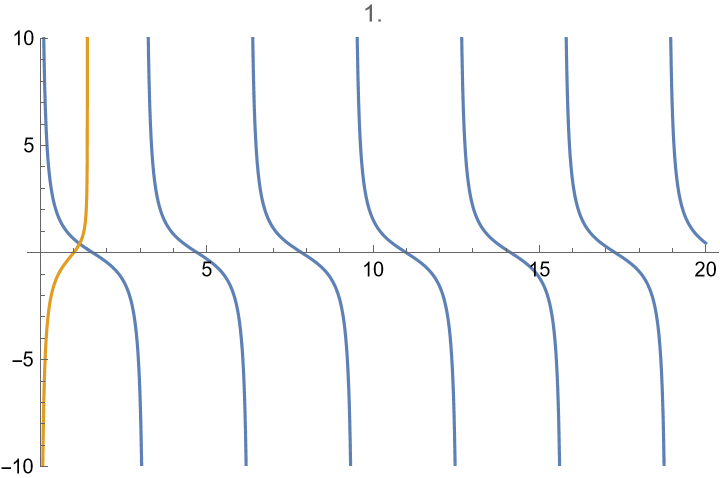
\includegraphics[width=.6\textwidth]{plots/case1.png}
    \end{center} 
    which shows that we have one soliton solution. As we increase $p$ a new soliton emerges around $p = 6$, meaning that there are two solitons. 
    \begin{center}
        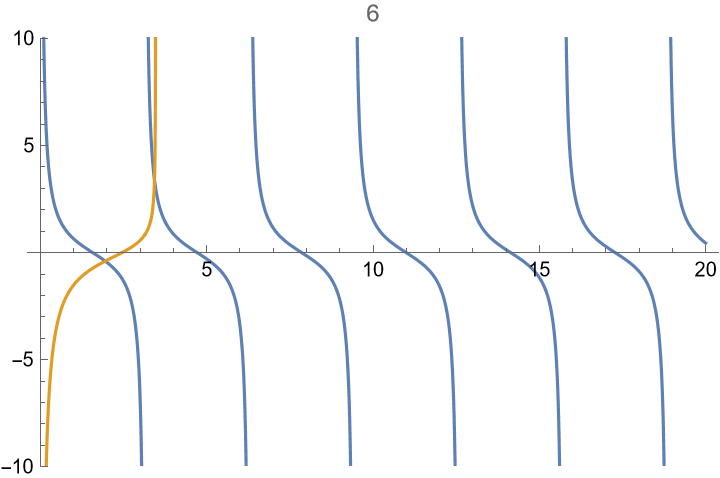
\includegraphics[width=.6\textwidth]{plots/case2.png}
    \end{center} 
    Continuing to increase $p$, $a(k)$ gains another soliton around $p=22$ which gives three solitons. 
    \begin{center}
        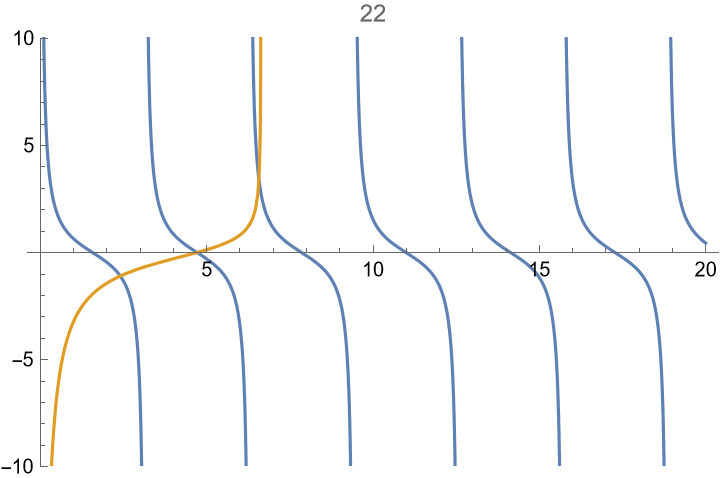
\includegraphics[width=.6\textwidth]{plots/case3.png}
    \end{center} 
    Noting that the fourth soliton only emerges around $p=49$, we have that number of solitons corresponding to the given initial condition increases as the value of $p = 2L^2d$ increases but we see that the rate of new emerging solitons decreases as $p$ gets large.
    \begin{center}
        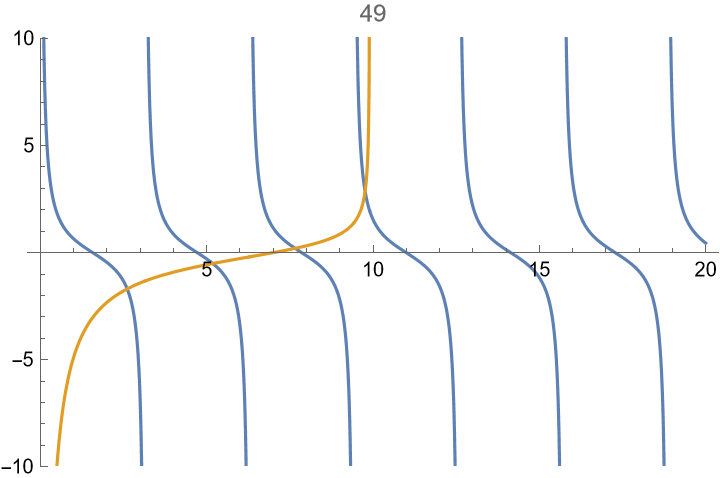
\includegraphics[width=.6\textwidth]{plots/case4.png}
    \end{center} 
    \noindent
    {\bf What happens for negative $d$:}
    In the case when $d < 0$, 
    \[ 
        a(i\kappa) = -\frac{e^{-2 \kappa  L} \left(\frac{\left(d-2 \kappa ^2\right) \sin \left(2 L \sqrt{d-\kappa ^2}\right)}{\sqrt{d-\kappa ^2}}-2 \kappa  \cos \left(2 L \sqrt{d-\kappa ^2}\right)\right)}{2 \kappa } = 0.
    \]
    will be strictly positive since we have already shown that $\sqrt{d - \kappa^2} \in \C \implies a(i\kappa) > 0$. Thus there are no soliton solutions when $d < 0$. 

    \noindent
    {\bf Limit as L goes to 0:}
    Using Mathematica we can evaluate
    \[ \lim_{L \to 0} a(k) = 1 - \frac{i \alpha}{2k} = 1 + \frac{\alpha}{2ik} = \frac{\alpha + 2 i k}{2 i k},\]
    under the transformation $2dL = \alpha$. Considering that taking the limit as $L \to 0$ is similar to restricting the initial condition to a delta function $u(x,0) = \alpha \delta(x)$, it is to no surprise that
    \[ \lim_{L \to 0} a(k) = \frac{\alpha + 2 i k}{2 i k},\]
    based off the work we did in class.
\end{solution}

%----------------------------------------------------------------------------------------------------%
%\vskip 20pt
\newpage

%---------------%
%---Problem 4---%
%---------------%

%--status--$

\begin{problem}
    This is no problem.
\end{problem}

\begin{solution}
    \noindent
    The solution is left as an exercise for the reader.
\end{solution}

%----------------------------------------------------------------------------------------------------%
%\vskip 20pt
\newpage

%---------------%
%---Problem 5---%
%---------------%

%--status--$

\begin{problem}
    {\bf The Liouville equation}. Consider the horribly nonlinear PDE
\[
u_{xy}=e^u,
\]
known as Liouville's equation. Consider the transformation
\begin{align*}
v_x&=-u_x+\sqrt{2}e^{(u-v)/2},\\
v_y&=u_y-\sqrt{2}e^{(u+v)/2},
\end{align*}
where $u(x,y)$ satisfies Liouville's equation above.

\begin{enumerate}

\item [a] Find an equation satisfied by $v(x,y)$: $v_{xy}=\ldots$. Your right-hand side cannot have any $u$'s. Those should all be eliminated.
\item [b] Write down the general solution for $v(x,y)$ from the equation you obtained.

\item [c] Use this solution for $v$ in your B\"acklund transformation and solve for $u$, obtaining the general solution of the Liouville equation!

\end{enumerate}
\end{problem}

\begin{solution}
    Consider the Liouville's equation
    \[
    u_{xy}=e^u,
    \]
    and consider the transformation
    \begin{align*}
        v_x&=-u_x+\sqrt{2}e^{(u-v)/2},\\
        v_y&=u_y-\sqrt{2}e^{(u+v)/2},
    \end{align*}
    where $u(x,y)$ satisfies Liouville's equation above.
    \noindent
    \begin{enumerate}
        \item [a]
        First we wish to find an equation $v_{xy}$ that satisfies $v(x,y)$. First observe that we can rewrite $v_x$ as
        \[
            v_x =-u_x+\sqrt{2}e^{(u-v)/2} \implies
            u_x = -v_x + \sqrt{2}e^{(u-v)/2},
        \]
        and taking a $y$ derivative of this gives
        \begin{equation} \label{5-1}
            u_{xy} = -v_{xy} + \frac{\sqrt{2}}{2}e^{(u-v)/2}(u_y - v_y).
        \end{equation}
        Similarly we can rewrite $v_y$ as
        \[ 
            v_y = u_y - \sqrt{2}e^{(u+v)/2} \implies
            u_y = v_y + \sqrt{2}e^{(u+v)/2},
        \]
        and taking a $x$ derivative of this gives
        \begin{equation} \label{5-2}
            u_{yx} = v_{yx} + \frac{\sqrt{2}}{2}e^{(u+v)/2}(u_x + v_x).
        \end{equation}
        Setting \ref{5-1} and \ref{5-2} equal under the assumption that the mixed derivatives are equal gives,
        \begin{align}
            -v_{xy} + \frac{\sqrt{2}}{2}e^{(u-v)/2}(u_y - v_y) &= v_{yx} + \frac{\sqrt{2}}{2}e^{(u+v)/2}(u_x + v_x) \nonumber \\
            -2v_{xy} &= -\frac{\sqrt{2}}{2}e^{(u-v)/2}(u_y - v_y) + \frac{\sqrt{2}}{2}e^{(u+v)/2}(u_x + v_x) \nonumber \\ 
            4v_{xy} &= \sqrt{2}e^{(u-v)/2}(u_y - v_y) - \sqrt{2}e^{(u+v)/2}(u_x + v_x) \label{5-3}.
        \end{align}
        Recalling that our transformation gives
        \begin{align*}
            v_x&=-u_x+\sqrt{2}e^{(u-v)/2} \implies \sqrt{2}e^{(u-v)/2} = v_x + u_x\\
            v_y&=u_y-\sqrt{2}e^{(u+v)/2} \implies \sqrt{2}e^{(u+v)/2} = u_y - v_y,
        \end{align*}
        we are able to rewrite \ref{5-3} as
        \[
            4v_{xy} = (v_x + u_x)(u_y - v_y) - (u_y - v_y)(u_x + v_x) = 0.
        \]
        Therefore we have found that
        \[v_{xy} = 0.\]


        \item [b]
        Since $v_{xy} = 0$ we have that a general solution for $v(x,y)$ is of the form
        \[
            v(x,y) = f(x) + g(y),
        \]
        where $f(x)$ and $g(y)$ are arbitrary functions of $x$ and $y$ respectively.
        
        \item [c]
        Finally let's plug the general form $v$ back into the B\"acklung transformation and solve for $u$ to get a general solution to the Liouville equation. Plugging the general solution of $v$ into the transformation gives
        \[ 
            \begin{cases}
                v_x &= -u_x + \sqrt{2}e^{(u-f(x)-g(y))/2}\\
                v_y &= u_y - \sqrt{2}e^{(u+f(x)+g(y))/2}.
            \end{cases}
        \]
        To get an integration factor, let's rewrite the system as following
        \[ 
            \begin{cases}
                e^{-(u+f(x))/2}(u+f(x))_x &= \sqrt{2}e^{-g(y)/2}e^{-f(x)}\\
                e^{-(u - g(y))/2}(u - g(y))_y &= \sqrt{2}e^{f(x)/2}e^{g(y)}
            \end{cases},
        \]
        and after integrating we have
        \[ 
            \begin{cases}
                -2e^{-(u + f(x))/2} &= \sqrt{2}e^{-g(y)/2}\paren{\int e^{-f(x)}dx + c_1(y)}\\
                -2e^{-(u-g(y))/2} &= \sqrt{2}e^{f(x)/2}\paren{\int e^{g(y)}dy + c_2(x)},
            \end{cases}
        \]
        where $c_1$ and $c_2$ are integration constants. Next we can take the $\ln$ of both sides and rewrite the system as following
        \begin{align*}
            &\begin{cases}
                \frac{-u - f(x)}{2} &= \ln\paren{\frac{-1}{\sqrt{2}}e^{-g(y)/2}\paren{\int e^{-f(x)}dx + c_1(y)}}\\
                \frac{-u + g(y)}{2} &= \ln\paren{\frac{-1}{\sqrt{2}}e^{f(x)/2}\paren{\int e^{g(y)}dy + c_2(x)}}
            \end{cases}\\
            \implies &\begin{cases}
                u &= -2\ln\paren{\frac{1}{\sqrt{2}}} + g(y) -2\ln\paren{-\int e^{-f(x)}dx + c_1(y)} - f(x)\\
                u &=  -2\ln\paren{\frac{1}{\sqrt{2}}} - f(x) - 2\ln\paren{-\int e^{g(y)} dy + c_2(x)} + g(y)
            \end{cases}\\
            \implies &\begin{cases}
                u &= \ln(2) + g(y) -2\ln\paren{-\int e^{-f(x)}dx + c_1(y)} - f(x)\\
                u &=  \ln(2) - f(x) - 2\ln\paren{-\int e^{g(y)} dy + c_2(x)} + g(y)
            \end{cases}.
        \end{align*}
        Combining these equations gives the general solution of the Liouville equation to be
        \[ 
            u = \ln(2) + g(y) - f(x) - 2\ln\paren{-\int e^{-f(x)}dx - \int e^{g(y)}dy}.
        \]


    \end{enumerate}
\end{solution}

%----------------------------------------------------------------------------------------------------%
%\vskip 20pt
\newpage

%---------------%
%---Problem 6---%
%---------------%

%--status--$

\begin{problem}
    {\bf The sine-Gordon equation.} Consider the sine-Gordon equation
\[
u_{xt}=\sin u,
\]
also horribly nonlinear.

\begin{enumerate}

\item [a] Show that the transformation
\begin{align*}
v_x=u_x+2\sin \frac{u+v}{2},\\
v_t=-u_t-2\sin \frac{u-v}{2},
\end{align*}
is an {\em auto-B\"acklund transformation} for the sine-Gordon equation. In other words, $v$ satisfies the same equation as $u$.

\item [b] Let $u(x,t)$ be the simplest solution of the sine-Gordon equation. With this $u(x,y)$ solve the auto-B\"acklund transformation for $v(x,t)$, to find a more complicated solution of the sine-Gordon equation. Congratulations! You just found the one-soliton solution of the sine-Gordon equation.
\end{enumerate}

\end{problem}

\begin{solution}
    
    \noindent
    Consider the sine-Gordon equation
    \[
        u_{xt}=\sin u.
    \]
    \begin{enumerate}
        \item [a]
        We wish to show that the transformation
        \begin{align}
            v_x=u_x+2\sin \frac{u+v}{2}, \label{6-1}\\
            v_t=-u_t-2\sin \frac{u-v}{2}, \label{6-2}
        \end{align}
        is an {\em auto-B\"acklund transformation} for the sine-Gordon equation. In other words, $v$ satisfies the same equation as $u$. First let's take a $t$ derivative of \ref{6-1} to get
        \[
            v_{xt} = u_{xt} + \cos\paren{\frac{u+v}{2}}(u_t + v_t)
        \]
        and plugging in the sine-Gordon equation gives
        \[
            v_{xt} = \sin u + \cos\paren{\frac{u+v}{2}}(u_t + v_t).
        \]
        Solving \ref{6-2} for $u_t$ and plugging it into the previous equation gives
        \begin{align*}
            v_{xt} &= \sin u + \cos\paren{\frac{u+v}{2}}(-2\sin\paren{\frac{u-v}{2}} - v_t + v_t)\\ 
            &= \sin(u) - 2\cos\paren{\frac{u+v}{2}}\sin\paren{\frac{u-v}{2}}\\
            &= \sin(u)-2\paren{\frac{\sin\paren{\frac{u+v+u-v}{2}}-\sin\paren{\frac{u+v-u+v}{2}}}{2}}\\
            &= \sin(u) - \sin(u) + \sin(v)\\
            &=\sin(v).
        \end{align*}
        Thus we have That
        \[v_{xt} = \sin(v),\]
        which verifies that $v$ satisfies the same equation as $u$ and thus the transformation given by \ref{6-1} and \ref{6-2} is an auto-B\"acklung transformation for the sine-Gordon equation.

        \item [b]
        Next we wish to find the one-soliton solution of the sine-Gordon equation. Let's begin by letting $u(x,t) = 0$ which is the simplest solution to the sine-Gordon equation. Then the auto-B\"acklung transformation becomes 
        \begin{align}
            v_x = 2\sin\paren{\frac{v}{2}} \label{6-3}\\
            v_t = -2\sin\paren{\frac{-v}{2}} \label{6-4}.
        \end{align}
        Observe that solving \ref{6-3} for $v$ gives
        \[ 
            \int \frac{v_x}{2\sin\paren{\frac{v}{2}}}dx = \int 1 dt.
        \]
        Using Mathematica to evaluate this integral gives
        \[
            \ln\paren{\tan\paren{\frac{v}{4}}} = t + c_1(x)
            \implies v = 4 \tan^{-1}(e^{t+c_1(x)}),
        \]
        where $c_1$ is an integration constant.
        Noticing that \ref{6-4} can be rewritten in the form of \ref{6-3} since 
        \[ 
            v_t = -2\sin\paren{\frac{-v}{2}} = 2\sin\paren{\frac{v}{2}} = v_x,
        \]
        gives that solving \ref{6-4} for $v$ yields
        \[ 
            v = 4 \tan^{-1}(e^{t+c_2(t)}),
        \]
        where $c_2$ is an integration constant. Furthermore, since $v_x = v_t$, $c_1 = $ and $c_2 = t$. Therefore
        \[ 
            v(x,t) = 4 \tan^{-1}\paren{e^{x+t}},
        \] 
        which is the one-soliton solution of the sine-Gordon equation. 

    \end{enumerate}
\end{solution}

%----------------------------------------------------------------------------------------------------%
%\vskip 20pt
\newpage

\end{document}